\subsection{NVD Case Study}
\label{sec:evaluation_nvd}
The U.S. National Institute of Standards and Technology (NIST) maintains the National Vulnerability Database (NVD) ~\footnote{https://nvd.nist.gov/}, an online database of publicly reported software vulnerabilities, with over 79,000 vulnerabilities dating back to 1988. Vulnerability reporters assign each vulnerability a Common Vulnerability Scoring System (CVSS) score and associated CVSS base metrics, according to the scheme defined in the CVSS guide~\cite{mell2007complete}.  

\subsubsection{Data selection}
\label{sec:evaluation_nvd_selection}
 We translate the CVSS metrics into the terms of our model constructs and measurements. For each structural model construct, we present our metric associations and the rationale behind them.
 
\textbf{Asset Impact}
CVSS has three impact metrics: Confidentiality Impact, Integrity Impact, and Availability Impact. The impact metrics are measurements of the degree of loss of confidentiality, integrity, and availability caused by the exploited vulnerability~\cite{mell2007complete}. Each impact metric is measured on the following scale of impact to the system:
	\begin{itemize}
		\item 'None' indicates no impact, 
		\item 'Partial' indicates partial impact, and 
		\item 'Complete' indicates 'Complete' impact.  
	\end{itemize}
We model each Impact metric as a component of Asset Value, theorizing that confidentiality, integrity, and availability impacts change based on the usage context in which the software is run, e.g. the value of the assets managed. We translate None/Partial/Complete to an ordinal scale (values 1,2,3 increasing with impact) to model increasing CIA impact risk.

\textbf{Software Risk}
\label{sec:evaluation_nvd_selection_risk}
The CVSS Access Vector, Access Complexity, and Authentication metrics capture how a vulnerability is accessed and whether or not extra conditions are required to exploit it.~\cite{mell2007complete}. We translate these metrics into the terms of our model constructs and measurements. For each metric, we now quote the CVSS guide definition, and give a rationale for the associations we have defined:
\begin{itemize}
	\item Access Vector - measures how the vulnerability is exploited, in terms of network distance. Values:
	\begin{itemize}
		\item 'Local' requires the attacker to have physical access or an account on the system, \item 'Adjacent Network' requires access to the physical network on which the vulnerable software resides, and \item 'Network' requires only logical network acccess, e.g. remote access. 
	\end{itemize}
	We model Access Vector Risk as a component of Software Risk, theorizing that the vector value changes based on design choices made by the software development team. We translate the CVSS Access Vector values (1,2,3, increasing with network distance) to an ordinal scale to model increasing `Access Vector Risk'.
	\item Access Complexity - measures the complexity of attack required to exploit a vulnerability once an attacker has gained access. Values: 
	\begin{itemize}
		\item 'High' indicates specialized/elevated access is required to exploit the vulnerability, 
		\item 'Medium' indicates that some access is required to exploit the vulnerability, and \item 'Low' indicates that the vulnerability can be exploited with default/no special access.  
	\end{itemize}
	We model Access Complexity Risk as a component of Software Risk, theorizing that the complexity value changes based on design choices made by the software development team. We translate the CVSS Access Complexity  to an ordinal scale (values 1,2,3, increasing with ease of access) to model increasing `Access Complexity Risk'.
	\item Authentication - measures the number of times an attacker must authenticate to exploit a vulnerability. Values: 
	\begin{itemize}
		\item 'Multiple' indicates an attacker must authenticate two or more times to exploit the vulnerability, 
		\item 'Single' indicates that an attacker must authenticate once to exploit the vulnerability, and 
		\item 'None' indicates that the vulnerability can be exploited without authenticating.  
	\end{itemize}
	We model Authentication as a component of Software Risk, theorizing that the authentication requirement changes based on design choices made by the software development team. We translate CVSS Authentication values to an ordinal scale (values 1,2,3, increasing with ease of authentication) to model increasing `Authentication Risk'.
\end{itemize}
  
\textbf{Adherence}
Kaminsky et al. ~\cite{kaminsky2011showing} hypothesized that software quality has increased over the past decade. To test their hypothesis, they fuzzed ten years of Microsoft Office software releases, confirming that software quality had improved over the previous decade, as measured by crash counts per software release over time. We adapt their hypothesis to the security realm, modeling security practice adherence via the passage of time. We take the year each vulnerability is reported as indicative of the state of security practice adherence at the time the vulnerability was reported. We define an `adherence' metric for each vulnerability as the difference, in years, between the vulnerability's publication date and the initial year in the NVD database. If software quality, presumed to be caused by security practice adherence, is increasing, we would expect to see a negative covariance between the Adherence construct and the SoftwareRisk construct. 

\textbf{Outcomes}
We obtain a metric for Outcomes by counting per-project, per-year vulnerabilities. We treat each unique software name in the NVD records as a distinct project, and sum all vulnerabilities for a project, reflecting our theorized post-release vulnerability count metric. We group each project by its (software) name, and by publication year, taking the mean of the remaining CVSS metrics to represent that project/publication year. 
% plot vuln count over time
% plot cvss score average
% plot three impact metrics
% plot three access metrics	

\textbf{NVD Data Examples}
To illustrate how data is prepared for use in SEM estimation, Table \ref{tab:nvd_data_examples} presents data from an example project. The Amazon flexible payments service experienced two vulnerabilities in 2012. The table presents the original data rows, the translated version of each row, and the project summary row, assembled from the translated rows. The project summary row is used in SEM estimation.

\begin{table}
	\begin{center}	
		\caption{NVD Original and Summarized Data for Example Project (Amazon flexible\_payments\_service)}
		\label{tab:nvd_data_examples}
		\begin{scriptsize}
			\begin{tabular}{p{3cm}p{1.5cm}p{1cm}p{1.5cm}p{1cm}p{1cm}}
				&&&&&\\[-1.8ex]\hline 
				\hline &&&&\\[-1.8ex] 
				Field & Original & Translated & Original & Translated & Project Summary \\
				\hline &&&&&\\[-1.8ex] 				
				CVE Count &  1 & 1 & 1 & 1 & 2\\
				&&&&& 1.10\\
				Pub Year & 2012 & 2012 & 2012 & 2012 & 2012\\
				Adherence & & 5.26 & & 5.26 & 5.26 \\				
				CVSS Auth & NONE & 1 & NONE & 1 & 1 \\
				Access Vector & NETWORK & 3 & NETWORK & 3 & 3 \\
				Access Complexity & MEDIUM & 2 & MEDIUM & 2 & 2 \\
				Conf Impact & PARTIAL & 2 & PARTIAL & 2 & 2\\
				Integ Impact & PARTIAL & 2 & PARTIAL & 2 & 2\\
				Avail Impact & NONE & 1 & NONE & 1 & 1 \\
				\hline &&&&&\\[-1.8ex] 		
			\end{tabular}
		\end{scriptsize}
	\end{center}
\end{table}
			
			
\subsubsection{Data collection}
We collected the entire NVD dataset as of February 2017, but limit our analysis to complete years, from the year 2001 to 2016. The dataset includes vulnerabilities dating to 1988, but years prior to 2001 had relatively low activity. We measured activity for a year as the ratio of vulnerabilities reported that year to the average vulnerabilities per year over the NVD history. Activity first exceeded half of the overall average in 2001. We show NVD Vulnerability counts per year in Figure ~\ref{fig:nvd_vulns_year}.

\begin{figure}
	\centering
	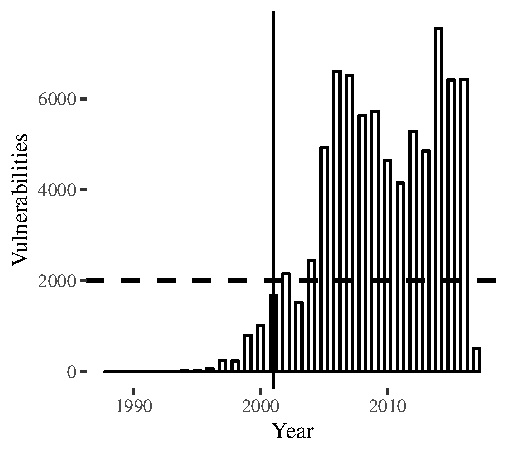
\includegraphics[width=.6\columnwidth]{nvd_vulns_year}
	\caption{NVD Vulnerability Count by Year}
	\label{fig:nvd_vulns_year}
\end{figure}
% stargazer(rtrunc)
% Table created by stargazer v.5.2 by Marek Hlavac, Harvard University. E-mail: hlavac at fas.harvard.edu
% Date and time: Sun, Feb 26, 2017 - 22:57:53
\begin{table}[!htbp] \centering 
	\caption{NVD Project Demographics} 
	\label{tab:nvd_demog} 
	\begin{small}
	\begin{tabular}{@{\extracolsep{5pt}}lccccc} 
		\\[-1.8ex]\hline 
		\hline \\[-1.8ex] 
		Statistic & \multicolumn{1}{c}{N} & \multicolumn{1}{c}{Mean} & \multicolumn{1}{c}{St. Dev.} & \multicolumn{1}{c}{Min} & \multicolumn{1}{c}{Max} \\ 
		\hline \\[-1.8ex] 
		CVECount & 10,622 & 4.311 & 5.241 & 2 & 49 \\ 
		logCVECount & 10,622 & 1.466 & 0.533 & 1.099 & 3.912 \\ 
		cvss\_score & 10,621 & 6.139 & 1.429 & 1.200 & 10.000 \\ 
		adherence & 10,621 & 4.678 & 1.007 & 0.225 & 6.532 \\ 
		cvss\_auth & 10,622 & 2.905 & 0.224 & 0.000 & 3.000 \\ 
		cvss\_access\_vector & 10,622 & 2.794 & 0.486 & 0.000 & 3.000 \\ 
		cvss\_access\_complexity & 10,622 & 2.577 & 0.409 & 0.000 & 3.000 \\ 
		cvss\_conf\_impact & 10,622 & 1.833 & 0.504 & 0.000 & 3.000 \\ 
		cvss\_integ\_impact & 10,622 & 1.902 & 0.467 & 0.000 & 3.000 \\ 
		cvss\_avail\_impact & 10,622 & 1.833 & 0.552 & 0.000 & 3.000 \\ 
		\hline \\[-1.8ex] 
	\end{tabular} 
		\end{small}
	
\end{table} 

\subsubsection{Estimation}

Combining the structural and measurement models we have defined with the CVSS data collected from the NVD database, we have the model definition, expressed in lavaan syntax: 

\begin{equation}
\begin{split}
	SoftwareRisk &=\sim cvss\_access\_vector \\ 
	&+ cvss\_access\_complexity + cvss\_auth\\
	AssetImpact &=\sim cvss\_conf\_impact\\
	&+ cvss\_integ\_impact + cvss\_avail\_impact\\
	Outcomes &=\sim logCVECount\\
	Adherence &=\sim adherence\\
	Outcomes &\sim SoftwareRisk + Adherence + AssetValue\\
	SoftwareRisk &\sim Adherence\\
\end{split}
\end{equation}		

\subsubsection{Model Fit} 
In terms of global fit, the fit index results for the initial NVD model were outside the range of standard fit criteria thresholds, as shown in the NVD column of Table \ref{tab:results_fit_all}. 

\subsubsection{Re-specification}
The base adherence and CVE Count metrics had variances two magnitudes larger than the other variables. We scaled adherence, and took the log of CVE Count to bring them within range of the other variables. The variation among the 18,000+ projects with exactly one vulnerability caused numeric problems for the estimation algorithm, and we elected to treat the group as outliers and drop them from consideration. After the exclusions, 6695 projects remained in the analyzed dataset.

The re-specified model (post-rescaling and outlier exclusion) had global fit characteristics within the traditional fit criteria thresholds, as shown in the Respecified NVD column of Table \ref{tab:results_fit_all}. We present the parameter estimates for the Respecified NVD model in the results, and discuss the implications in Section \ref{sec:case_nvd_discussion}.

\subsubsection{Reporting Results}
\label{sec:case_nvd_results}

Table \ref{tab:results_fit_all} presents the fit measure results for the NVD  and Respecified NVD models (as well as for the other case study models). We report the estimated parameter values, unstandardized, for the Respecified NVD structural and measurement models in Table \ref{tab:results_nvd}. We present the standardized parameter estimates, and the residuals, in the context of the full structural and measurement models in Figure \ref{fig:nvd_model_respecified_estimates}.

\begin{table*}
	\begin{center}	
		\caption{Global Fit Measures and Results}
			\label{tab:results_fit_all}
			\begin{tabular}{p{3cm}p{1cm}|p{2cm}p{2cm}p{2cm}}
				\\[-1.8ex]\hline 
				\hline \\[-1.8ex] 
				Fit Measure & Threshold & NVD	& Respecified NVD & Respecified CII  \\
				\hline \\[-1.8ex] 				
				Number of observations &  & $10621$  & $10621$ & $343$  \\				
				Model chi-square &  & $2759.88$ & 1068.25 & $259$  \\				
				Model d.f. &  & $17$ & $18$ & $52$  \\		
				Model p-value & $\leq 0.01$ & $0.0$ & $0.0$ & $0.0$  \\
				RMSEA & $\leq 0.10$ &  $0.12$ &  $0.07$ & $0.108$   \\
				CFI & $> 0.90$ & $0.83$ & $0.93$  & $0.702$  \\
				SRMR & $< 0.08$ & $0.08$ & $0.06$ & $0.08$  \\
				\hline \\[-1.8ex] 				
			\end{tabular}
	\end{center}
\end{table*}

\begin{table}
	\begin{center}	
		\caption{NVD Respecified Model Results}
		\label{tab:results_nvd}
		\begin{tabular}{l|rrrr}
				\\[-1.8ex]\hline 
				\hline \\[-1.8ex] 
			\textit{Latent Variables}:  & & & & \\  
			$\sim$ Measured variables& Estimate & Std.Err & z$-$value & $P(>|z|)$ \\
				\hline \\[-1.8ex]
			$SoftwareRisk =\sim$  & & & & \\                                   
			cvss\_ccss\_vctr   & 1.000 & &  & \\                             
			cvss\_ccss\_cmpl &  $-$0.166 &   0.035 &  $-$4.86 &   0.000\\
			cvss\_auth     &   $-$1.498  &  0.164  & $-$9.125   & 0.000\\
			$AssetImpact =\sim$     & & & & \\                                    
			cvss\_conf\_mpct   & 1.000     & & & \\                       
			cvss\_intg\_mpct   & 0.797   & 0.011 & 70.746 &   0.000 \\
			cvss\_aval\_mpct  &  0.872   & 0.013 & 67.584   & 0.000 \\
			$Outcomes =\sim$    & & & & \\                                     
			logCVECount     &  1.000  & & & \\                          
			$Adherence =\sim$   & & & & \\                                      
			adherence    &     1.000        & & & \\                    
			Regressions:  & & & & \\  
			%& Estimate & Std.Err & z$-$value & $P(>|z|)$ \\
			$Outcomes \sim$         & & & & \\                                     
			SoftwareRisk   &  1.092 &   0.162 & 6.754 &   0.000 \\
			%Adherence       &  $-$2.84  &  6.829  &  -0.468  &  0.640\\
			AssetImpact     &   0.062  &  0.013  &  4.907 &   0.00\\
			$SoftwareRisk \sim$        & & & & \\                                  
			Adherence     &    0.044 &   0.005  &  9.465 &   0.000\\
			Covariances:  & & & & \\  
			%& Estimate & Std.Err & z$-$value & $P(>|z|)$ \\
			$AssetValue \sim\sim$          & & & & \\                                 
			Adherence      &  $-$0.017  &  0.005 &  $-$3.590 &   0.000\\
		\end{tabular}
	\end{center}
\end{table} 

\begin{figure*}
	\centering
	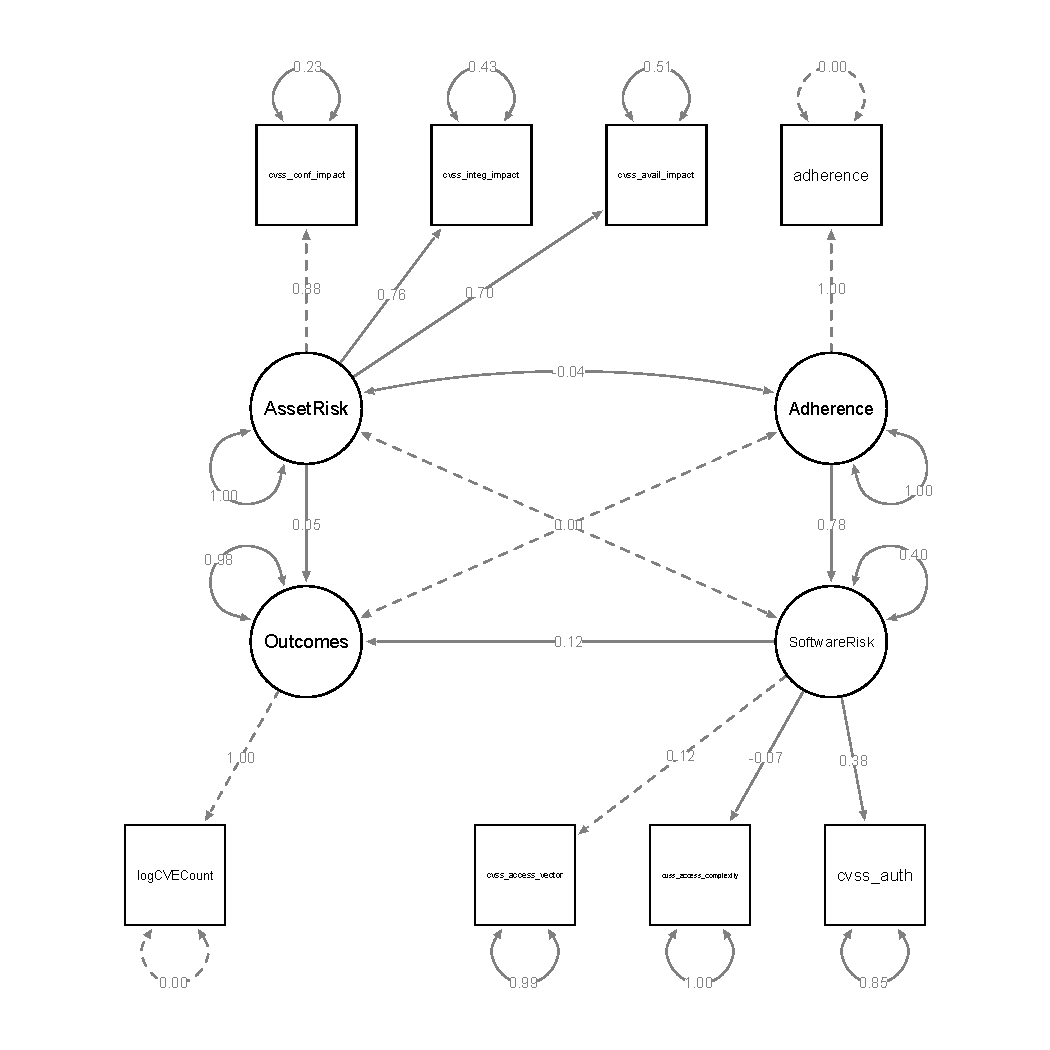
\includegraphics[width=.6\textwidth]{NVD_Respecified_SEM_Model.pdf}
	\caption{Respecified NVD Model}
	\label{fig:nvd_model_respecified_estimates}
\end{figure*}

Interpreting the (standardized) parameter estimates in terms of our hypothesized construct relationships, we have the following:
\begin{itemize}
	\item  Asset Impact is positively associated (0.05) with Security Outcomes, as hypothesized.
	\item Software Risk is positively associated (0.12) with Security Outcomes, as hypothesized. 
	\item Practice Adherence is positively associated (0.78) with Software Risk, contrary to what we hypothesized. 
\end{itemize}	
All three relationships were statistically significant. 

We plot how the three impact risk scores change over time in Figure \ref{fig:nvd_vulns_impact}, and the CVSS access risk scores in Figure \ref{fig:nvd_vulns_auth}. 	
		
\begin{figure}
	\centering
	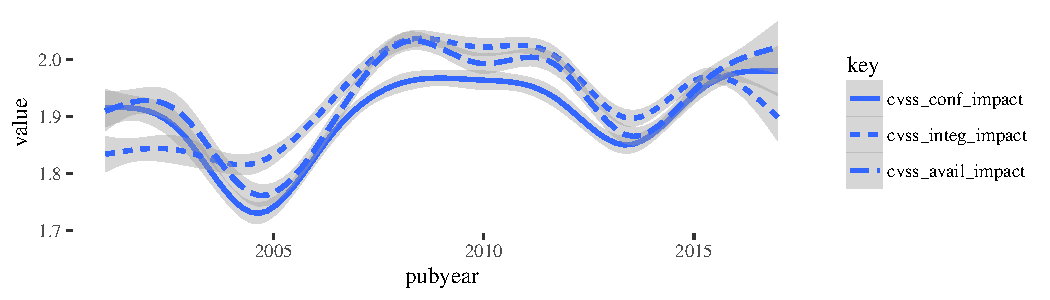
\includegraphics[width=\columnwidth]{nvd_cvss_impact}
	\caption{NVD CVSS Impact Risk by Year}
	\label{fig:nvd_vulns_impact}
\end{figure}

\begin{figure}
	\centering
	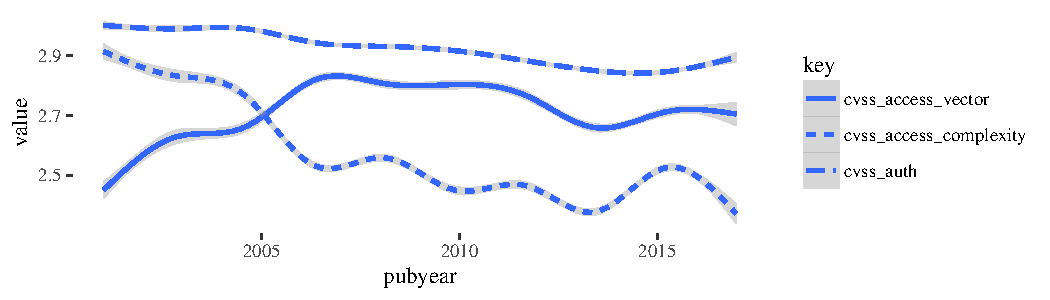
\includegraphics[width=\columnwidth]{nvd_cvss_auth}
	\caption{NVD CVSS Access Control Risk by Year}
	\label{fig:nvd_vulns_auth}
\end{figure}
